\documentclass[conference]{IEEEtran}

\usepackage{amsmath,amssymb}
\usepackage{booktabs}
\usepackage{graphicx}
\usepackage{hyperref}
\usepackage{placeins}
\usepackage{xcolor}
\usepackage{url}

\graphicspath{{figures/}}
\hypersetup{
  colorlinks=true,
  linkcolor=black,
  citecolor=black,
  urlcolor=blue
}

\title{Comparative Study of FLIP, APIC, and PolyPIC Transfers for Particle--Grid Fluid Simulation}

\author{
\IEEEauthorblockN{Qinzhe Hu \quad Yan Shao \quad Baihan Deng}
}

\begin{document}
\maketitle

\begin{abstract}
This paper compares three particle--grid transfer schemes for fluid simulation: FLIP, APIC, and PolyPIC. All methods are evaluated under a shared Taichi-based framework with identical grid resolution, boundary handling, particle generation, rendering style, and scene definitions. The study uses two representative three-dimensional scenarios, dam break and liquid pouring, and evaluates the methods using kinetic-energy evolution, visual behavior, and a controlled runtime benchmark. The results show that PolyPIC has the largest integrated kinetic energy in the dam-break scene, while APIC and PolyPIC produce smoother and lower-energy behavior than FLIP in the continuously driven pouring scene. The runtime measurements confirm the expected complexity ordering: FLIP is fastest, APIC is slower due to affine transfer state, and PolyPIC is slowest due to higher-order polynomial transfer state.
\end{abstract}

\begin{IEEEkeywords}
fluid simulation, FLIP, APIC, PolyPIC, particle-in-cell, Taichi, experimental validation
\end{IEEEkeywords}

\section{Introduction}

Particle--grid hybrid methods are widely used for visually rich fluid simulation because they combine Lagrangian advection with structured grid operations for forces, pressure projection, and boundary handling. This design is common in computer graphics liquid simulation, where stable grid solvers and particle/grid coupling are often combined to balance robustness and visual detail~\cite{foster2001liquids,bridson}. However, different particle--grid transfer schemes can produce noticeably different dissipation, stability, and runtime behavior even when the surrounding simulator is otherwise identical.

This study is an experimental validation rather than a new fluid model. The goal is to isolate the transfer scheme as much as possible. The three algorithms are run with the same grid, scenes, particle initialization, boundaries, frame count, and plotting pipeline. The reported outputs include energy CSV files, rendered videos, visual screenshots, comparison figures, and runtime summaries.

The evaluation addresses three questions: (1) which method preserves kinetic energy most strongly in the shared scenarios; (2) whether the qualitative videos are consistent with the quantitative energy trends; and (3) how much runtime overhead APIC and PolyPIC introduce relative to baseline FLIP in this implementation.

\section{Related Work}

The Particle-In-Cell (PIC) family transfers information between Lagrangian particles and an Eulerian grid. FLIP, introduced by Brackbill and Ruppel~\cite{brackbill1986flip}, reduces the excessive dissipation of pure PIC by transferring grid velocity increments back to particles. Related graphics work has used particle/grid methods for granular and fluid-like materials~\cite{zhu2005sand}. FLIP is attractive for energetic liquids, but it may also retain noisy velocity components.

APIC augments particles with locally affine velocity information~\cite{jiang2015apic}. Instead of storing only a constant velocity per particle, APIC carries an affine matrix that represents first-order local velocity variation. This improves angular momentum behavior and transfer consistency, at the cost of extra particle state and implementation complexity.

PolyPIC generalizes this direction by representing higher-order polynomial local velocity functions on particles~\cite{fu2017polypic}. The method is motivated by preserving richer local flow structure during particle--grid transfers. In a compact implementation, this additional expressiveness must be balanced against stability controls and runtime cost.

\section{Methods}

\subsection{Shared Simulation Framework}

All algorithms are evaluated using the shared three-dimensional Taichi framework in the repository. Taichi is designed for high-performance spatial computation and provides the CUDA backend used in these experiments~\cite{hu2019taichi}. The common setup uses a grid resolution of $80 \times 100 \times 80$, cell size $\Delta x = 0.01$, two simulation substeps per rendered frame, and 300 output frames. The experiments use the \texttt{ratio\_970} convention for the FLIP/PIC blend parameter so that the branches can be compared under the same naming and output structure.

Two scenes are used. The dam-break scene initializes a dense water block near one side of the domain and observes the subsequent collapse and spread. The liquid-pouring scene initializes a stream-like incoming fluid source and therefore acts as a continuously driven test case.

\subsection{Transfer Schemes}

FLIP uses the change in grid velocity after force application and projection to update particle velocities. Let $G^n(\mathbf{x}_p)$ and $G^{n+1}(\mathbf{x}_p)$ denote interpolated grid velocities at the particle position before and after the grid solve, and let $V_{\mathrm{PIC}}^{n+1}(\mathbf{x}_p)$ be the direct PIC interpolation from the updated grid. The blended update used by the FLIP branch can be written as
\begin{equation}
\mathbf{v}_p^{n+1}
= (1-\alpha) V_{\mathrm{PIC}}^{n+1}(\mathbf{x}_p)
+ \alpha \left[\mathbf{v}_p^n + G^{n+1}(\mathbf{x}_p)-G^n(\mathbf{x}_p)\right],
\label{eq:flip}
\end{equation}
where $\alpha=0.97$ for the \texttt{ratio\_970} runs. This keeps more kinetic activity than pure PIC but can carry high-frequency velocity noise.

APIC stores an affine matrix for each particle. Locally, particle $p$ represents velocity as
\begin{equation}
\mathbf{u}_p(\mathbf{x})
= \mathbf{v}_p + \mathbf{C}_p(\mathbf{x}-\mathbf{x}_p),
\label{eq:apic-local}
\end{equation}
where $\mathbf{C}_p$ is the affine velocity matrix. During particle-to-grid transfer, nearby grid nodes receive mass-weighted momentum of the form
\begin{equation}
m_i\mathbf{v}_i
\mathrel{+}= w_{ip}m_p
\left[\mathbf{v}_p+\mathbf{C}_p(\mathbf{x}_i-\mathbf{x}_p)\right],
\label{eq:apic-p2g}
\end{equation}
with interpolation weight $w_{ip}$. During grid-to-particle transfer, the implementation reconstructs particle velocity and affine state from the projected grid velocity field, conceptually following
\begin{equation}
\begin{aligned}
\mathbf{v}_p^{n+1} &= \sum_i w_{ip}\mathbf{v}_i^{n+1},\\
\mathbf{C}_p^{n+1} &\approx \mathbf{B}_p\mathbf{D}_p^{-1}, \quad
\mathbf{B}_p = \sum_i w_{ip}\mathbf{v}_i^{n+1}
(\mathbf{x}_i-\mathbf{x}_p)^{T}.
\end{aligned}
\label{eq:apic-g2p}
\end{equation}
Here $\mathbf{D}_p = \sum_i w_{ip}(\mathbf{x}_i-\mathbf{x}_p)(\mathbf{x}_i-\mathbf{x}_p)^T$ is the local weighted second-moment matrix, with implementation-side regularization and limiting applied for robustness.
The implementation used for the full run includes finite-value guards and affine damping to prevent NaN growth.

PolyPIC stores higher-order local transfer information. A compact way to describe the intended local model is
\begin{equation}
\mathbf{u}_p(\mathbf{x})
= \sum_{|\boldsymbol{\beta}|\le k}
\mathbf{a}_{p,\boldsymbol{\beta}}
\phi_{\boldsymbol{\beta}}(\mathbf{x}-\mathbf{x}_p),
\label{eq:polypic}
\end{equation}
where $\phi_{\boldsymbol{\beta}}$ are local polynomial basis functions and $\mathbf{a}_{p,\boldsymbol{\beta}}$ are particle-carried coefficients. APIC corresponds to preserving first-order local variation; PolyPIC extends the idea to richer polynomial structure. In this evaluation, PolyPIC is treated as the high-order branch of the same framework and compared using identical output metrics.

\subsection{Metrics and Efficiency Benchmark}

For each rendered frame, the pipeline records kinetic energy and validates that the time series remains finite. Kinetic energy is computed as
\begin{equation}
E_k(t_f)=\frac{1}{2}\sum_p m_p \|\mathbf{v}_p(t_f)\|_2^2,
\label{eq:energy}
\end{equation}
and the reported energy AUC uses a trapezoidal approximation,
\begin{equation}
\mathrm{AUC}(E_k)\approx
\sum_{f=0}^{N-2}
\frac{E_k(t_f)+E_k(t_{f+1})}{2}(t_{f+1}-t_f).
\label{eq:auc}
\end{equation}
We summarize each method using initial kinetic energy, peak kinetic energy, final kinetic energy, final-to-peak ratio, and the integral of kinetic energy over the simulated time interval.

Runtime efficiency is measured separately from the rendered runs. FLIP, APIC, and PolyPIC are evaluated in a single batch benchmark on the \texttt{rtxp6000} partition. The allocation uses one NVIDIA RTX PRO 6000 Blackwell Server Edition GPU, 8 CPU cores, and 64 GB host memory; the GPU reports driver 580.126.20 and 97,887 MiB of device memory. Taichi CUDA is enabled with \texttt{TI\_ARCH=cuda}. Rendering and video export are disabled so that timing focuses on simulation work. Each method-scene pair is measured for three repetitions, and the first five frames are discarded to reduce JIT compilation and initialization effects. Particle throughput is reported using the particle-count estimate recorded in the benchmark logs, so it should be read as approximate implementation throughput rather than a fixed hardware peak. Relative speed is normalized against FLIP:
\begin{equation}
S_{\mathrm{method}}=\frac{T_{\mathrm{FLIP}}}{T_{\mathrm{method}}},
\label{eq:speedup}
\end{equation}
where $T$ is mean milliseconds per frame. Values below $1$ indicate slower runtime than FLIP.

\section{Results}

\subsection{Dam-Break Energy Behavior}

\begin{figure}[!t]
  \centering
  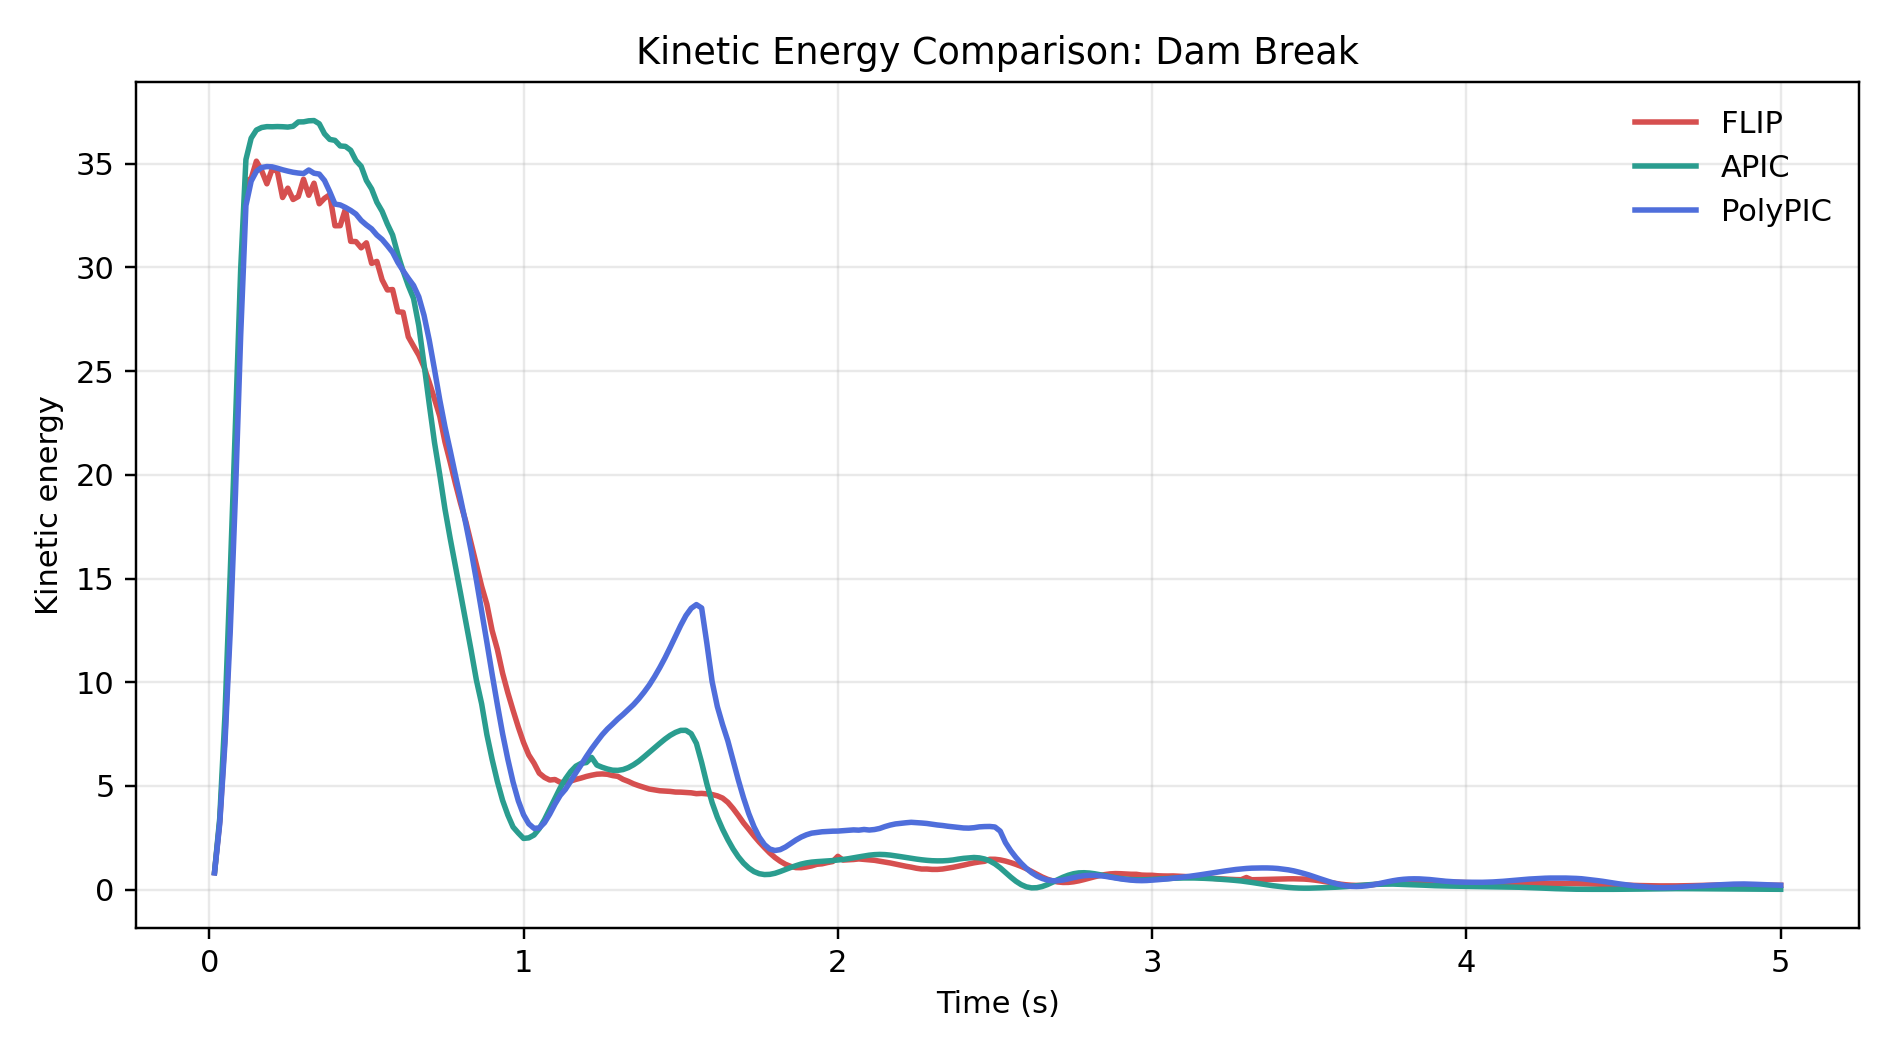
\includegraphics[width=\linewidth]{dam_break_kinetic_energy.png}
  \caption{Dam-break kinetic-energy evolution. PolyPIC keeps the largest integrated kinetic energy over the full run, while APIC reaches the highest peak and then dissipates more strongly.}
  \label{fig:dam-energy}
\end{figure}

\begin{table}[!t]
  \centering
  \footnotesize
  \setlength{\tabcolsep}{3pt}
  \caption{Dam-break energy summary. Final/Peak measures how much of each method's own peak kinetic energy remains at frame 300.}
  \label{tab:dam-energy}
  \begin{tabular}{lrrrr}
    \toprule
    Alg. & Peak & Final & AUC & Final/Peak \\
    \midrule
FLIP & 35.1273 & 0.2105 & 30.2746 & 0.60\% \\
APIC & 37.0836 & 0.0178 & 30.2771 & 0.05\% \\
PolyPIC & 34.8671 & 0.2117 & 34.1077 & 0.61\% \\
    \bottomrule
  \end{tabular}
\end{table}

In the dam-break scene, all three methods remain finite for the full run. PolyPIC has the largest integrated kinetic energy in this test; FLIP and PolyPIC have similar final-to-peak ratios, so the primary PolyPIC advantage is the larger energy AUC. APIC reaches the highest peak energy, but after stabilization it dissipates more strongly near the end of the run.

\begin{figure}[!t]
  \centering
  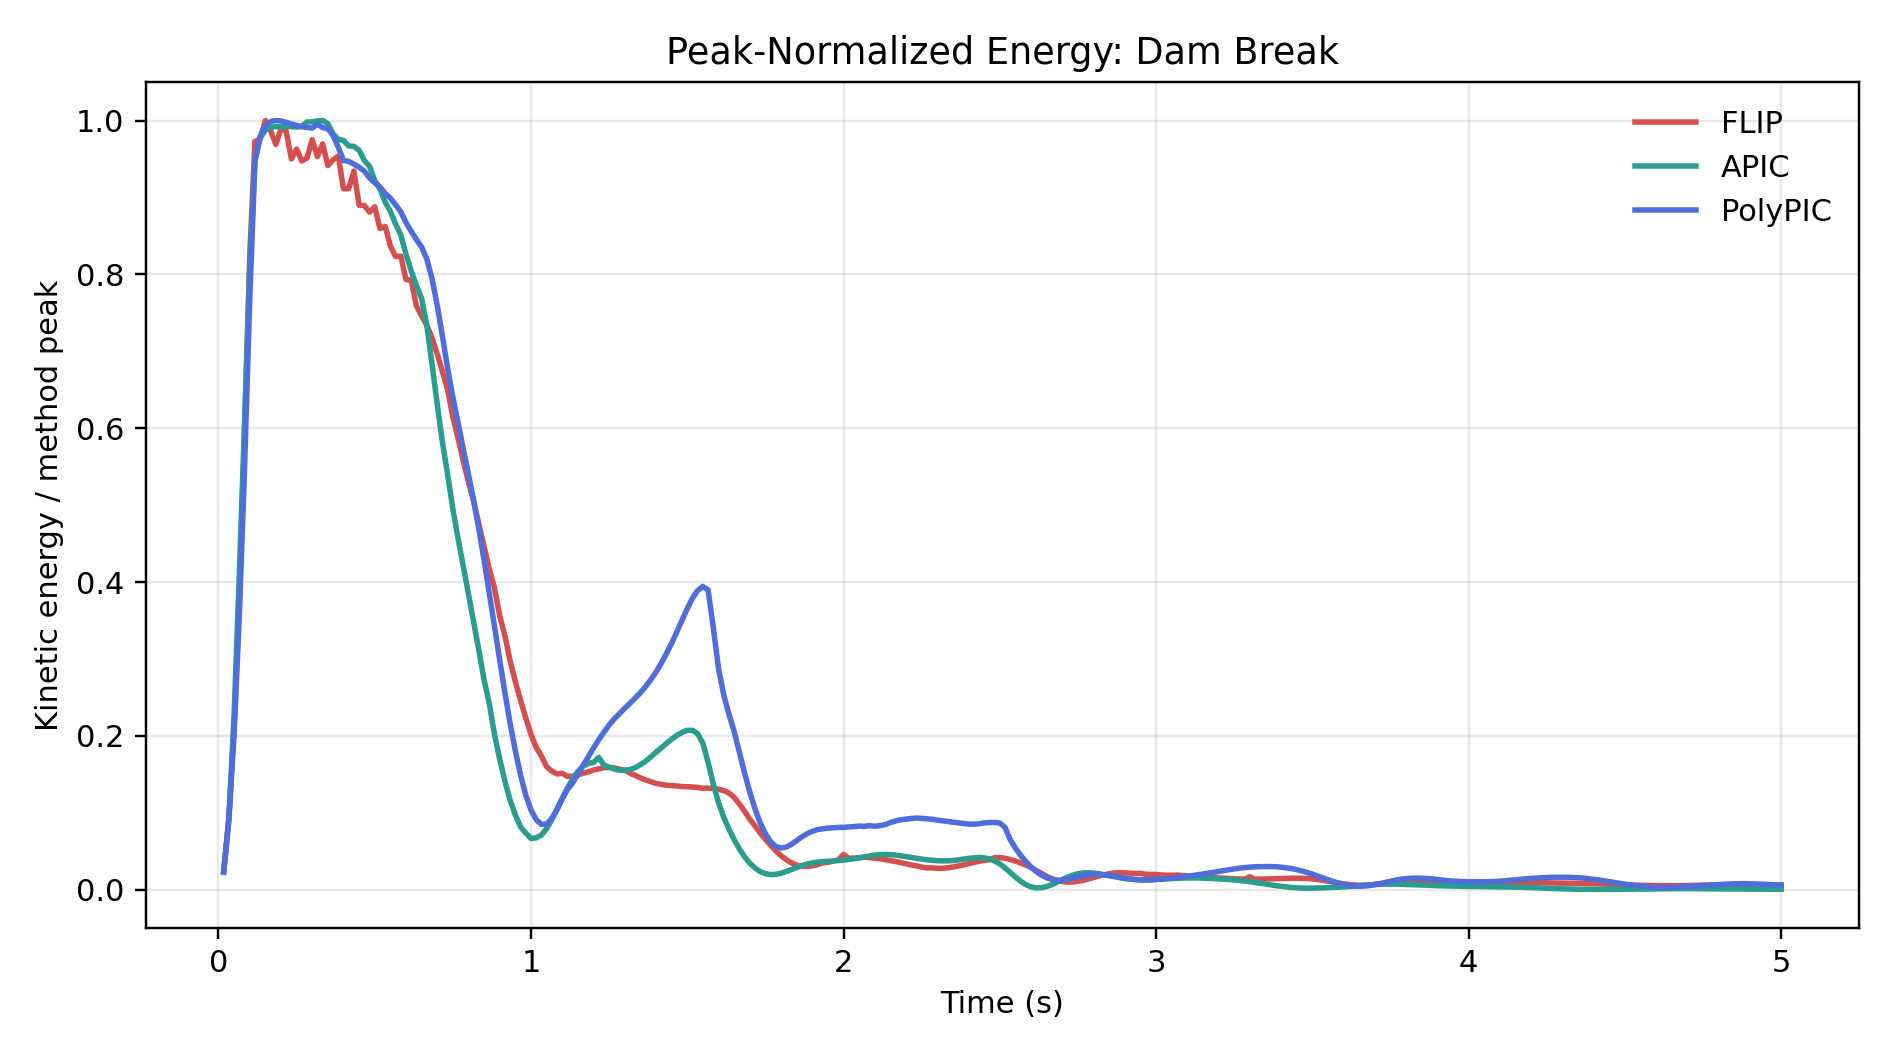
\includegraphics[width=\linewidth]{dam_break_energy_peak_normalized.png}
  \caption{Peak-normalized dam-break energy. Normalization removes scale differences and emphasizes dissipation after each method's own peak.}
  \label{fig:dam-normalized}
\end{figure}

\FloatBarrier

\subsection{Liquid-Pouring Energy Behavior}

\begin{figure}[!t]
  \centering
  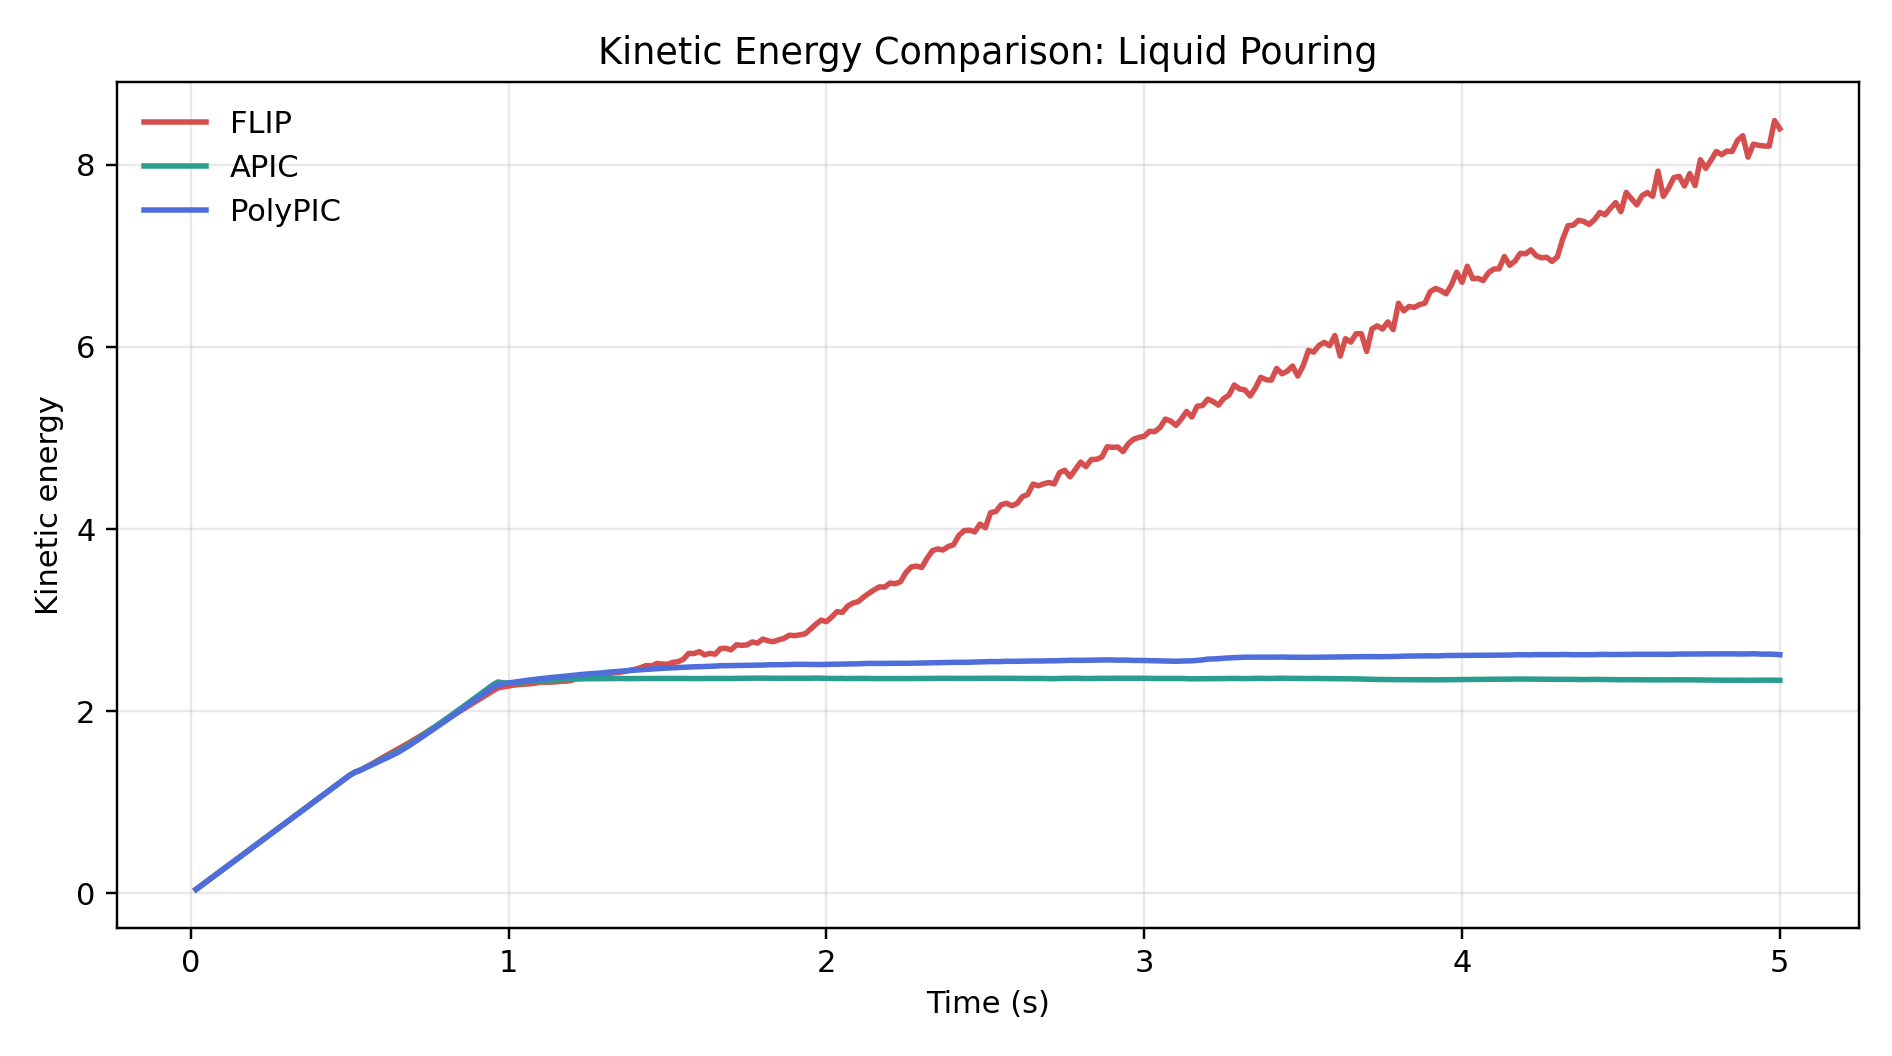
\includegraphics[width=\linewidth]{liquid_pouring_kinetic_energy.png}
  \caption{Liquid-pouring kinetic-energy evolution. FLIP reaches and maintains much higher kinetic energy than APIC and PolyPIC in the driven-source setup.}
  \label{fig:pour-energy}
\end{figure}

\begin{table}[!t]
  \centering
  \footnotesize
  \setlength{\tabcolsep}{3pt}
  \caption{Liquid-pouring energy summary. The lower APIC/PolyPIC values indicate more restrained transfer behavior in this forced scenario.}
  \label{tab:pour-energy}
  \begin{tabular}{lrrrr}
    \toprule
    Alg. & Peak & Final & AUC & Final/Peak \\
    \midrule
FLIP & 8.4851 & 8.3959 & 21.2332 & 98.95\% \\
APIC & 2.3630 & 2.3384 & 10.6397 & 98.96\% \\
PolyPIC & 2.6302 & 2.6197 & 11.4223 & 99.60\% \\
    \bottomrule
  \end{tabular}
\end{table}

In the liquid-pouring scene, FLIP produces substantially higher kinetic energy than APIC and PolyPIC. Because the scene is continuously driven, this should not be interpreted as directly superior behavior. High kinetic energy can indicate reduced dissipation, but it can also reflect noisy transfer or excessive momentum retention. APIC and PolyPIC give lower and smoother energy curves, with PolyPIC slightly above APIC in both peak and integrated energy.

\begin{figure}[!t]
  \centering
  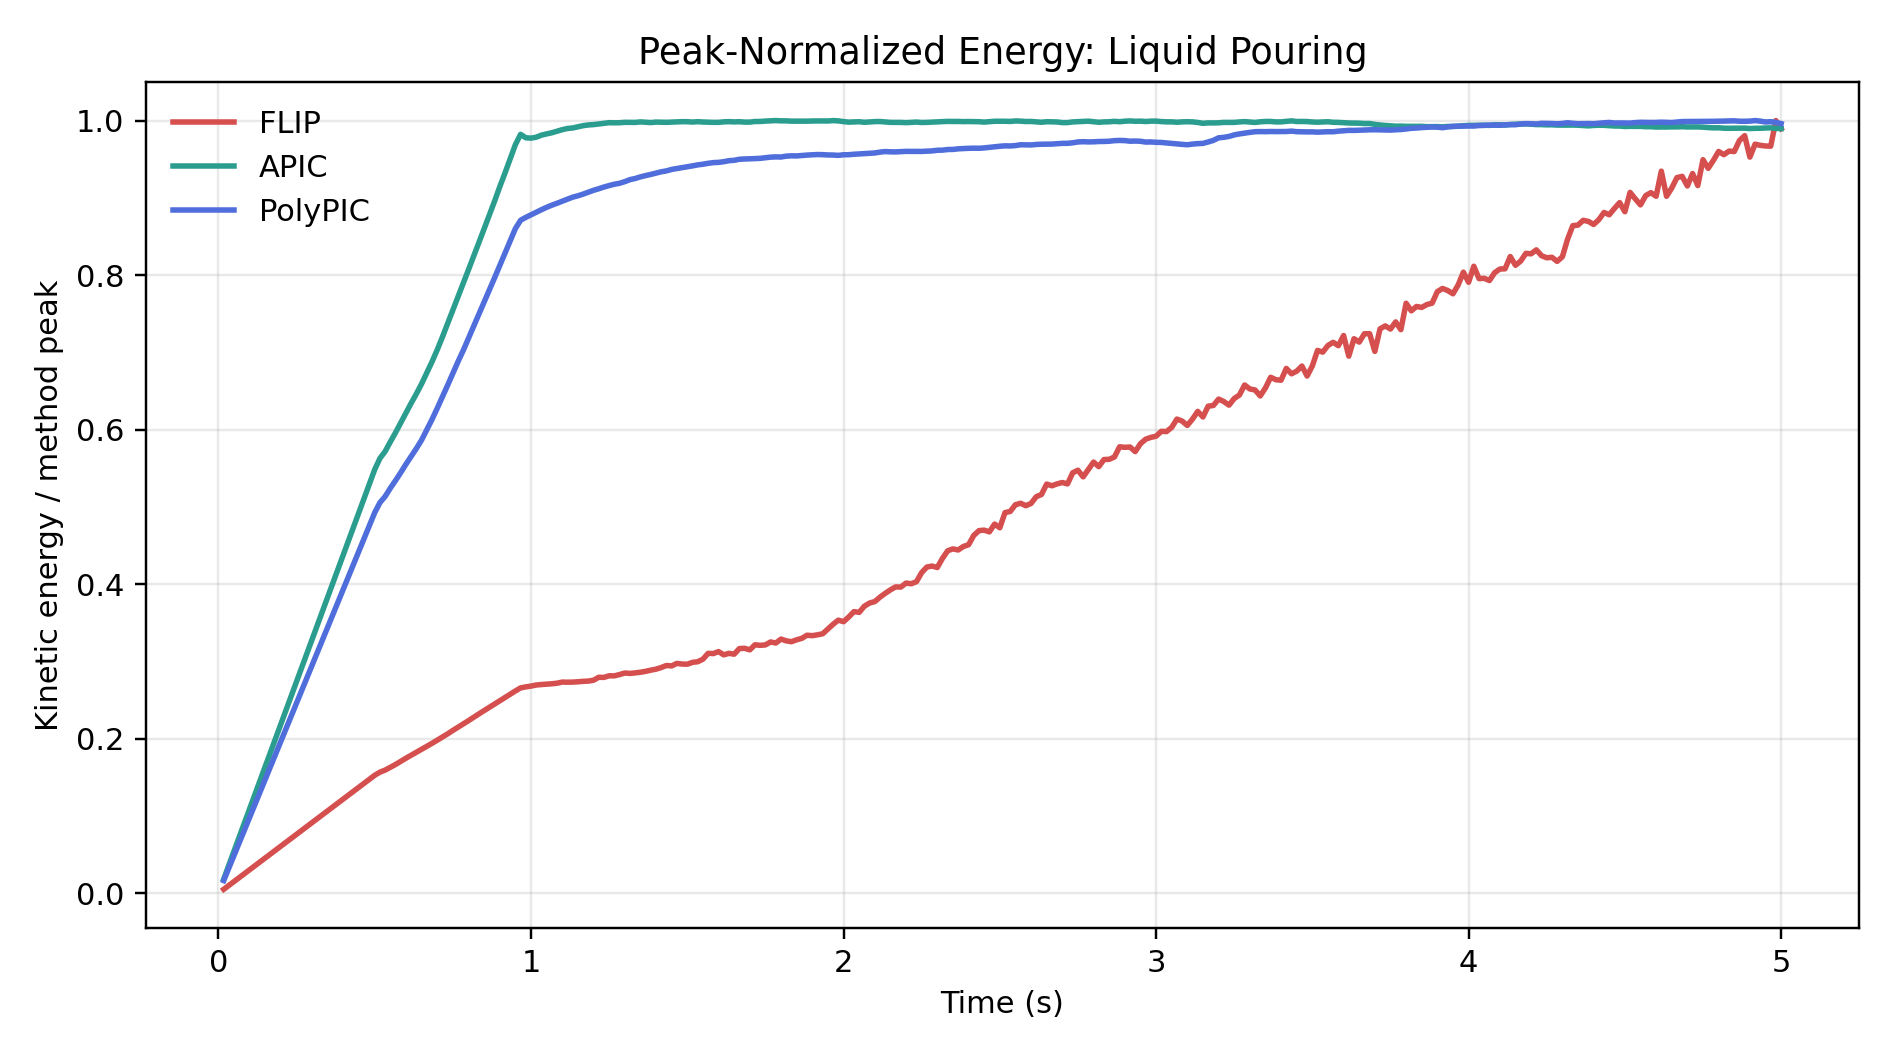
\includegraphics[width=\linewidth]{liquid_pouring_energy_peak_normalized.png}
  \caption{Peak-normalized liquid-pouring energy. APIC and PolyPIC remain close after their peaks, while FLIP maintains a much higher absolute kinetic-energy level.}
  \label{fig:pour-normalized}
\end{figure}

\begin{figure}[!t]
  \centering
  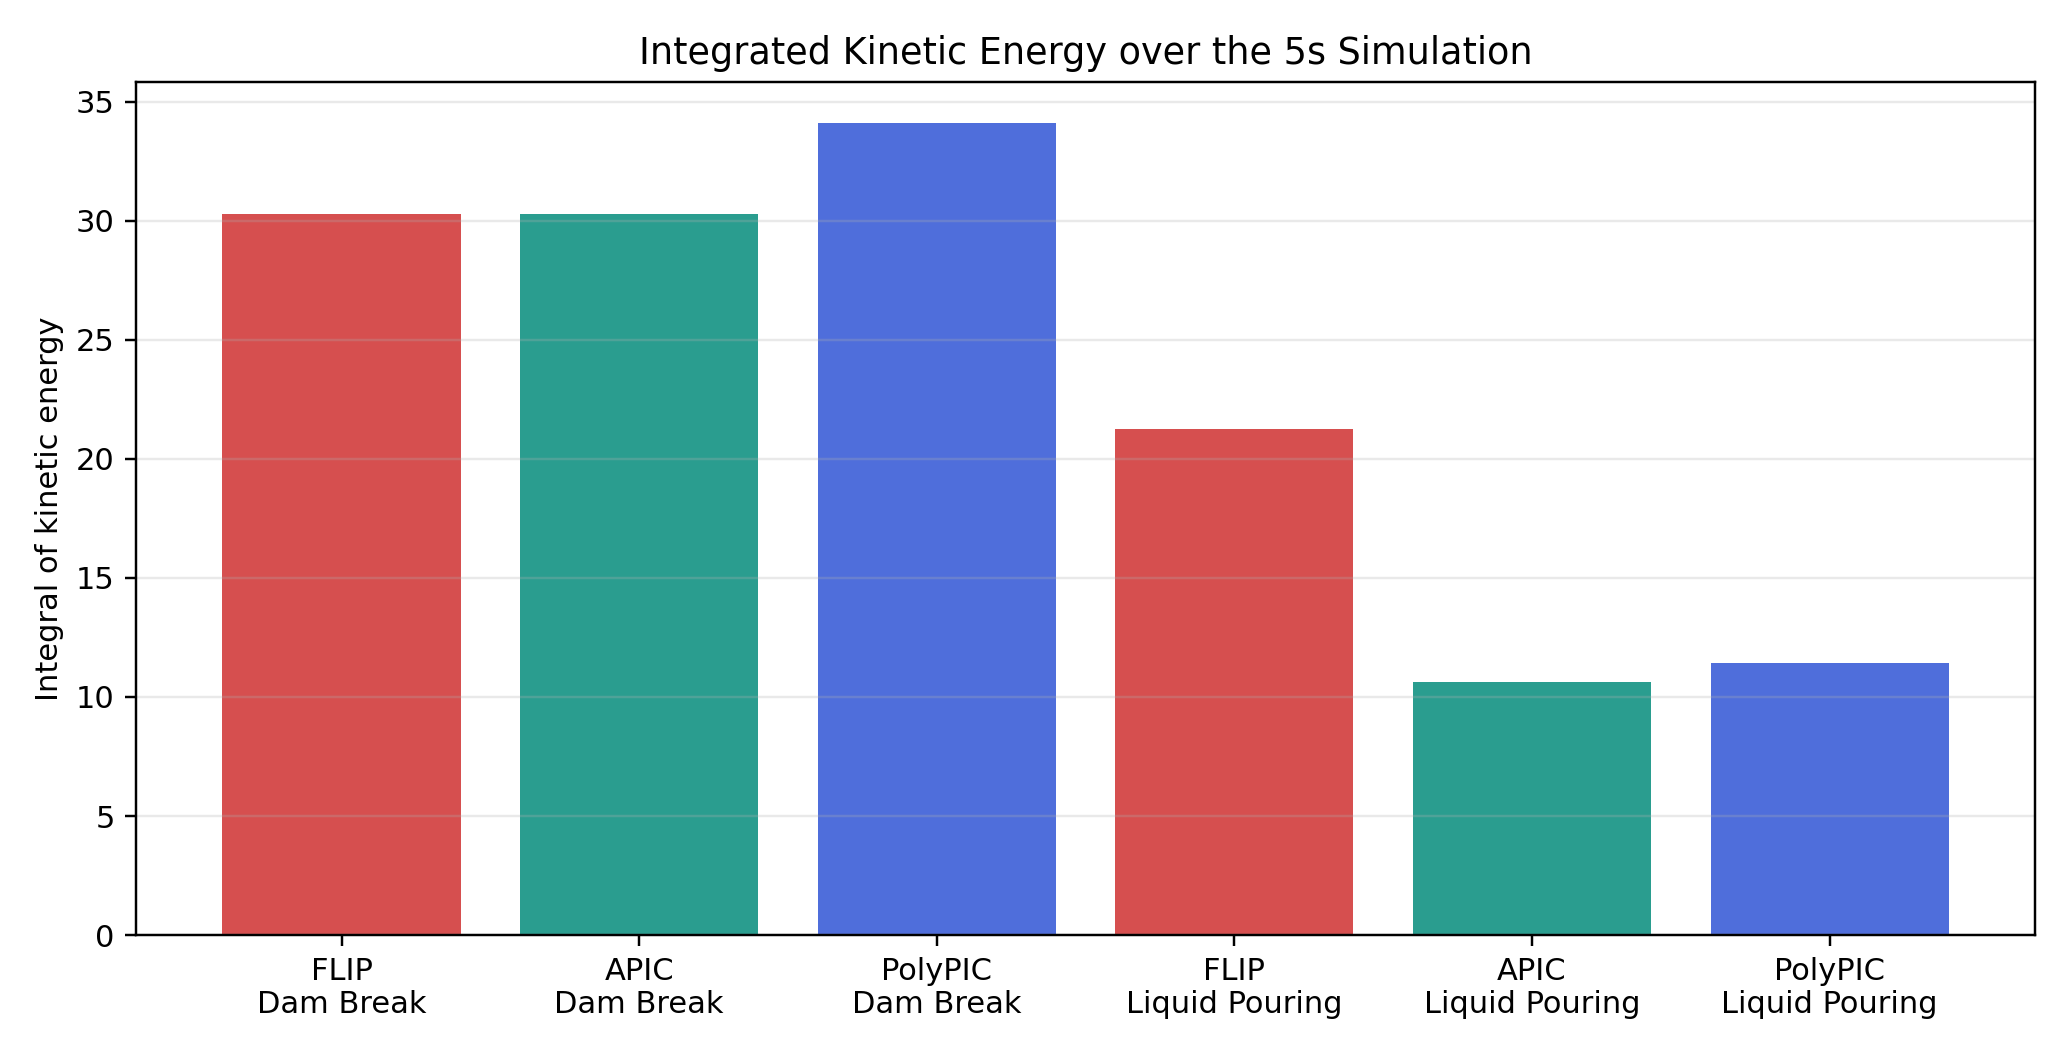
\includegraphics[width=\linewidth]{energy_auc_summary.png}
  \caption{Integrated kinetic energy across all method-scene pairs. This aggregate view highlights PolyPIC's dam-break advantage and FLIP's high-energy pouring behavior.}
  \label{fig:auc-summary}
\end{figure}

\FloatBarrier

\subsection{Visual Comparison}

\begin{figure*}[!t]
  \centering
  \begin{minipage}{0.49\textwidth}
    \centering
    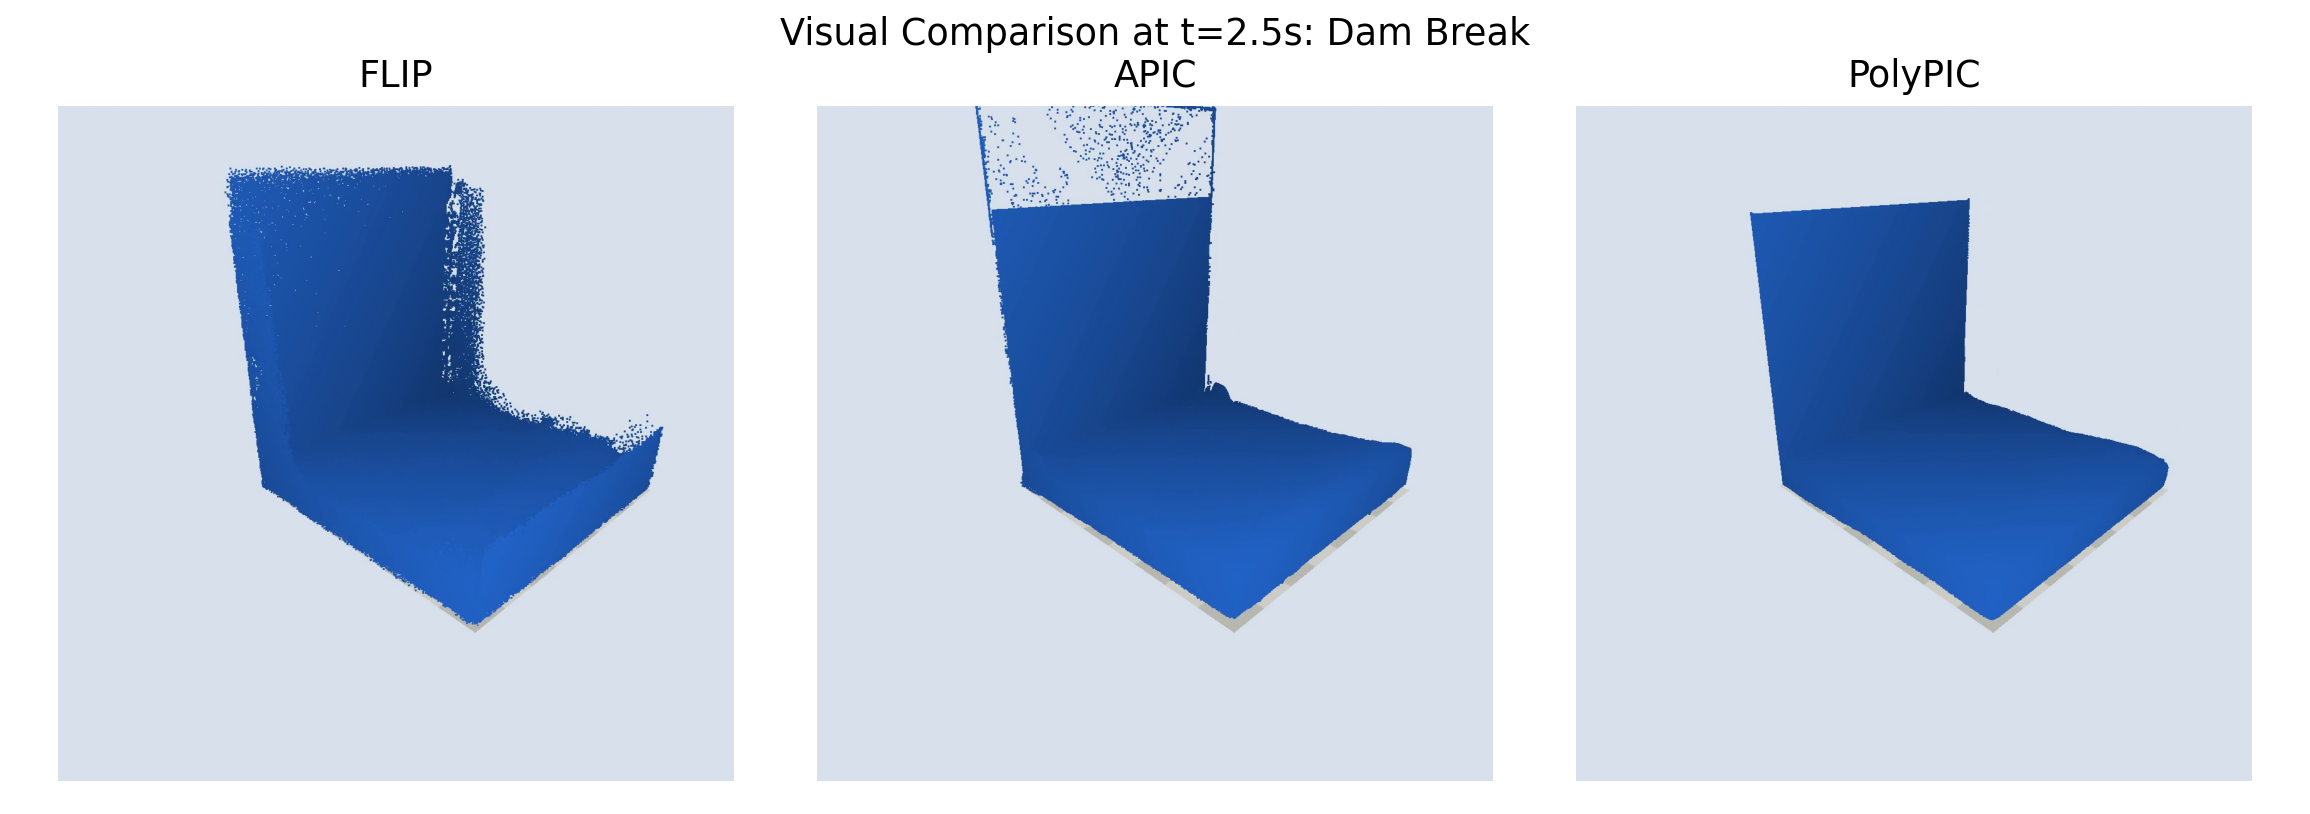
\includegraphics[width=\linewidth]{dam_break_visual_comparison.png}
    \vspace{-0.6em}
    \centerline{\footnotesize (a) Dam break at $t=2.5$s}
  \end{minipage}
  \hfill
  \begin{minipage}{0.49\textwidth}
    \centering
    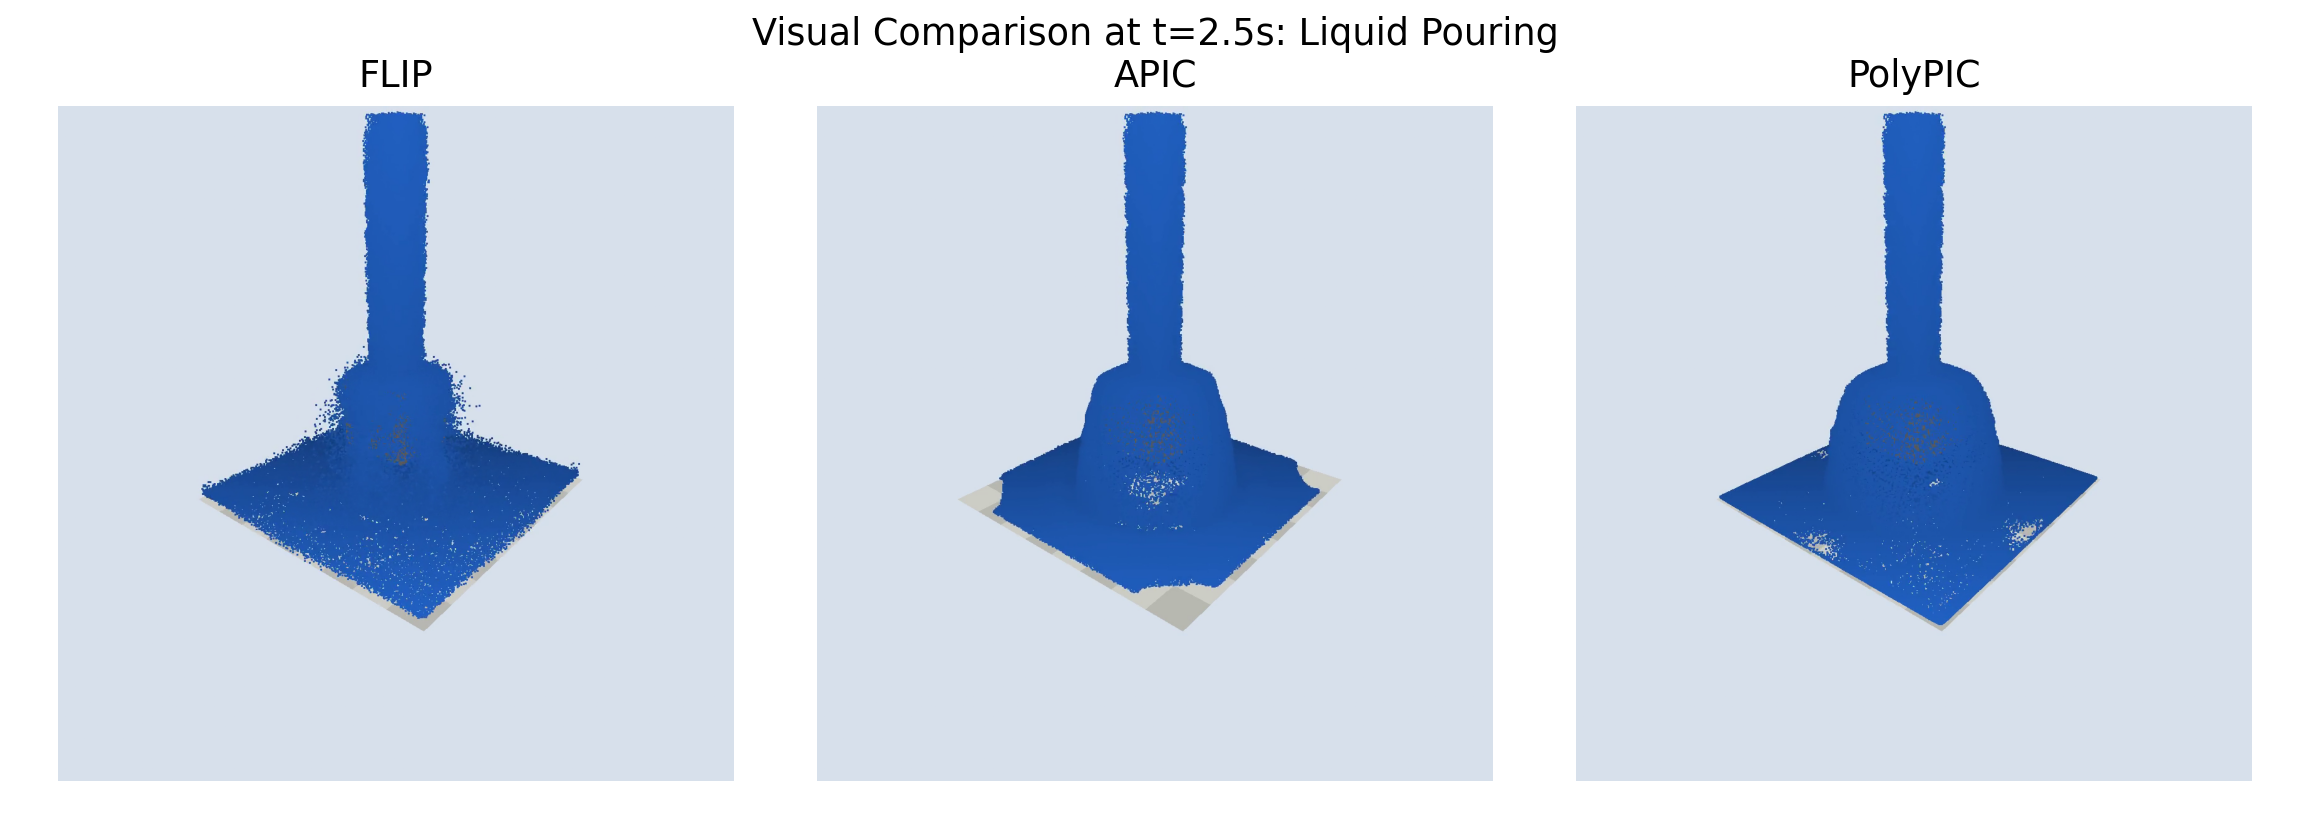
\includegraphics[width=\linewidth]{liquid_pouring_visual_comparison.png}
    \vspace{-0.6em}
    \centerline{\footnotesize (b) Liquid pouring at $t=2.5$s}
  \end{minipage}
  \caption{Visual comparison extracted from the committed videos. The screenshots use the same rendering style and sampling time across algorithms.}
  \label{fig:visual}
\end{figure*}

The visual outputs provide a qualitative check against the CSV traces. The dam-break videos show broadly similar large-scale motion, but the energy summaries indicate that PolyPIC retains more total kinetic activity over time. The pouring screenshots are consistent with the lower APIC and PolyPIC kinetic-energy curves in the driven source setup.

\FloatBarrier

\subsection{Efficiency}

\begin{figure}[!t]
  \centering
  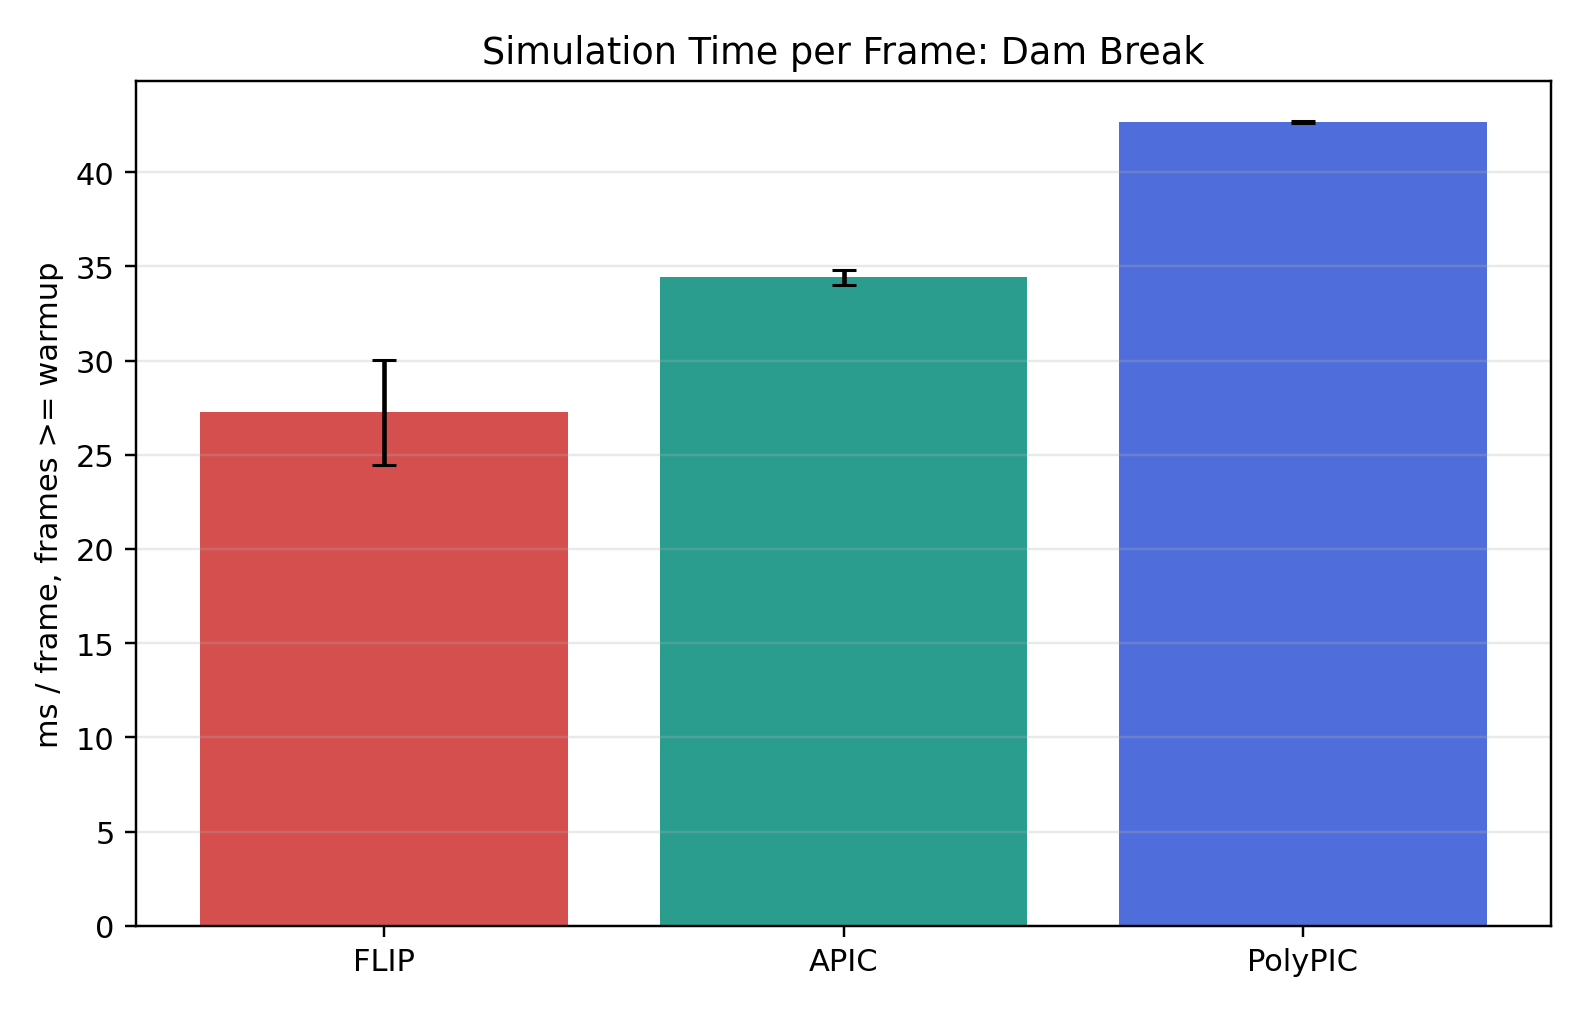
\includegraphics[width=\linewidth]{dam_break_efficiency_ms_per_frame.png}
  \caption{Dam-break simulation-only frame time. Rendering and video export are disabled.}
  \label{fig:dam-efficiency}
\end{figure}

\begin{table}[!t]
  \centering
  \footnotesize
  \setlength{\tabcolsep}{3pt}
  \caption{Dam-break efficiency benchmark. Speedup is normalized against FLIP.}
  \label{tab:dam-efficiency}
  \begin{tabular}{lrrrr}
    \toprule
    Alg. & Mean ms & P95 ms & Approx. Mpart/s & Speedup \\
    \midrule
FLIP & 27.246 & 35.070 & 75.91 & 1.00$\times$ \\
APIC & 34.417 & 45.385 & 59.67 & 0.79$\times$ \\
PolyPIC & 42.639 & 57.272 & 48.16 & 0.64$\times$ \\
    \bottomrule
  \end{tabular}
\end{table}

\begin{figure}[!t]
  \centering
  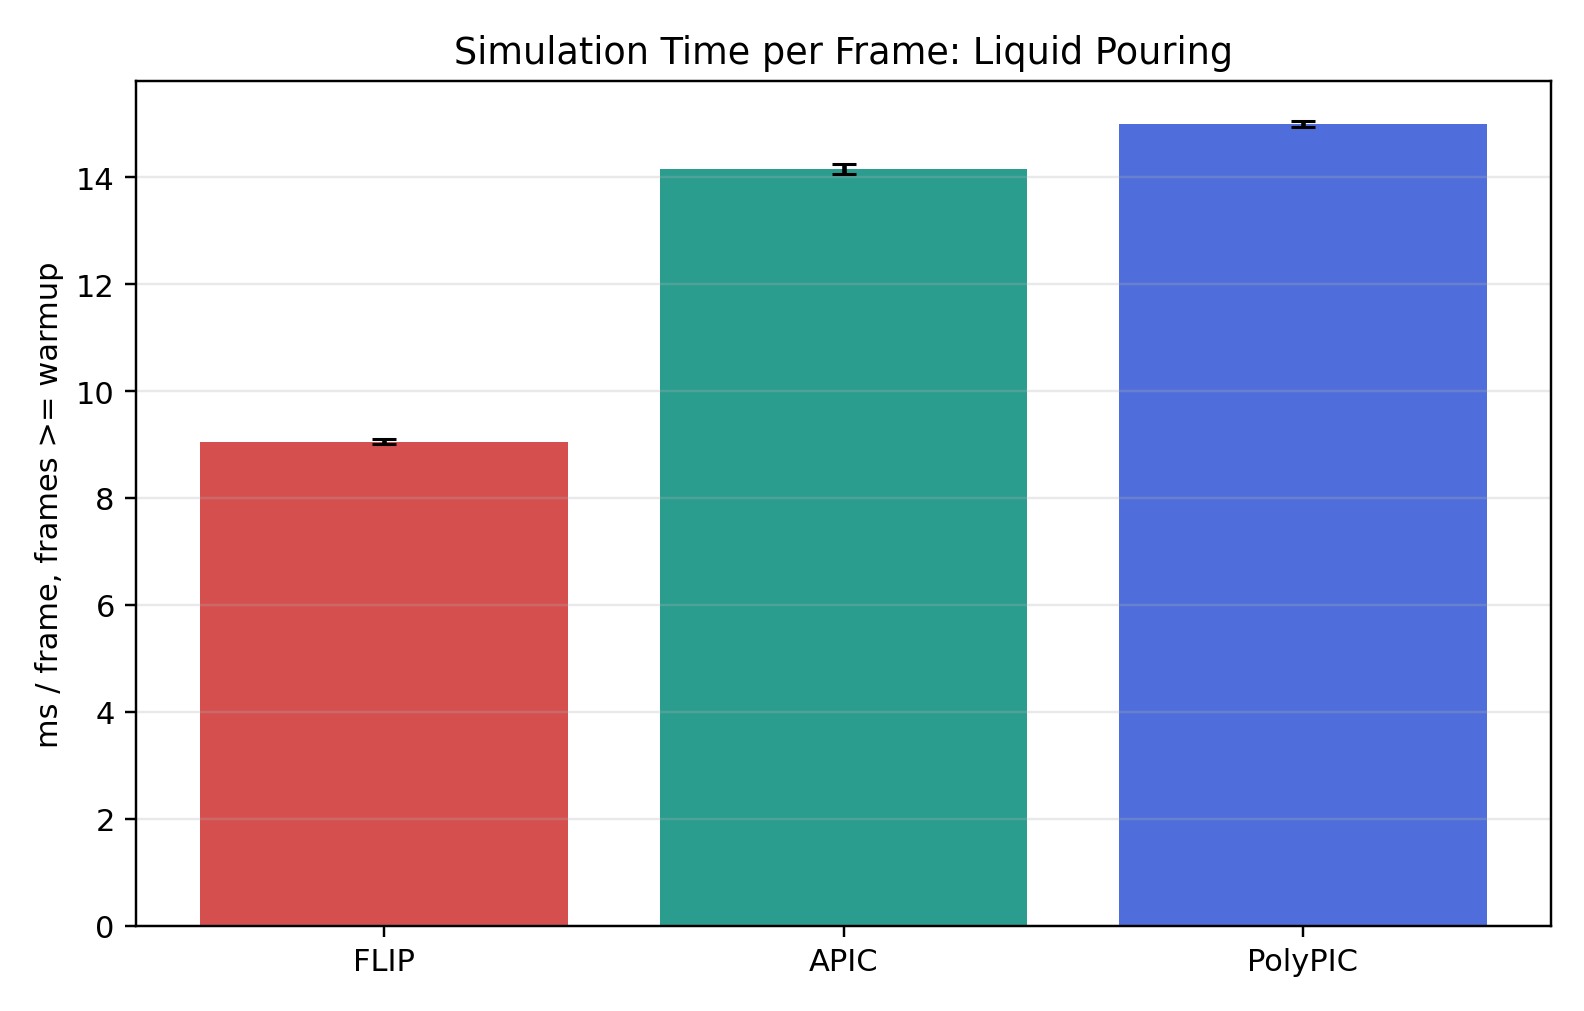
\includegraphics[width=\linewidth]{liquid_pouring_efficiency_ms_per_frame.png}
  \caption{Liquid-pouring simulation-only frame time. The same method ordering appears under the lower-particle-count scene.}
  \label{fig:pour-efficiency}
\end{figure}

\begin{table}[!t]
  \centering
  \footnotesize
  \setlength{\tabcolsep}{3pt}
  \caption{Liquid-pouring efficiency benchmark. Speedup is normalized against FLIP.}
  \label{tab:pour-efficiency}
  \begin{tabular}{lrrrr}
    \toprule
    Alg. & Mean ms & P95 ms & Approx. Mpart/s & Speedup \\
    \midrule
FLIP & 9.053 & 15.317 & 33.36 & 1.00$\times$ \\
APIC & 14.151 & 16.266 & 21.34 & 0.64$\times$ \\
PolyPIC & 14.988 & 16.972 & 20.15 & 0.60$\times$ \\
    \bottomrule
  \end{tabular}
\end{table}

\begin{figure}[!t]
  \centering
  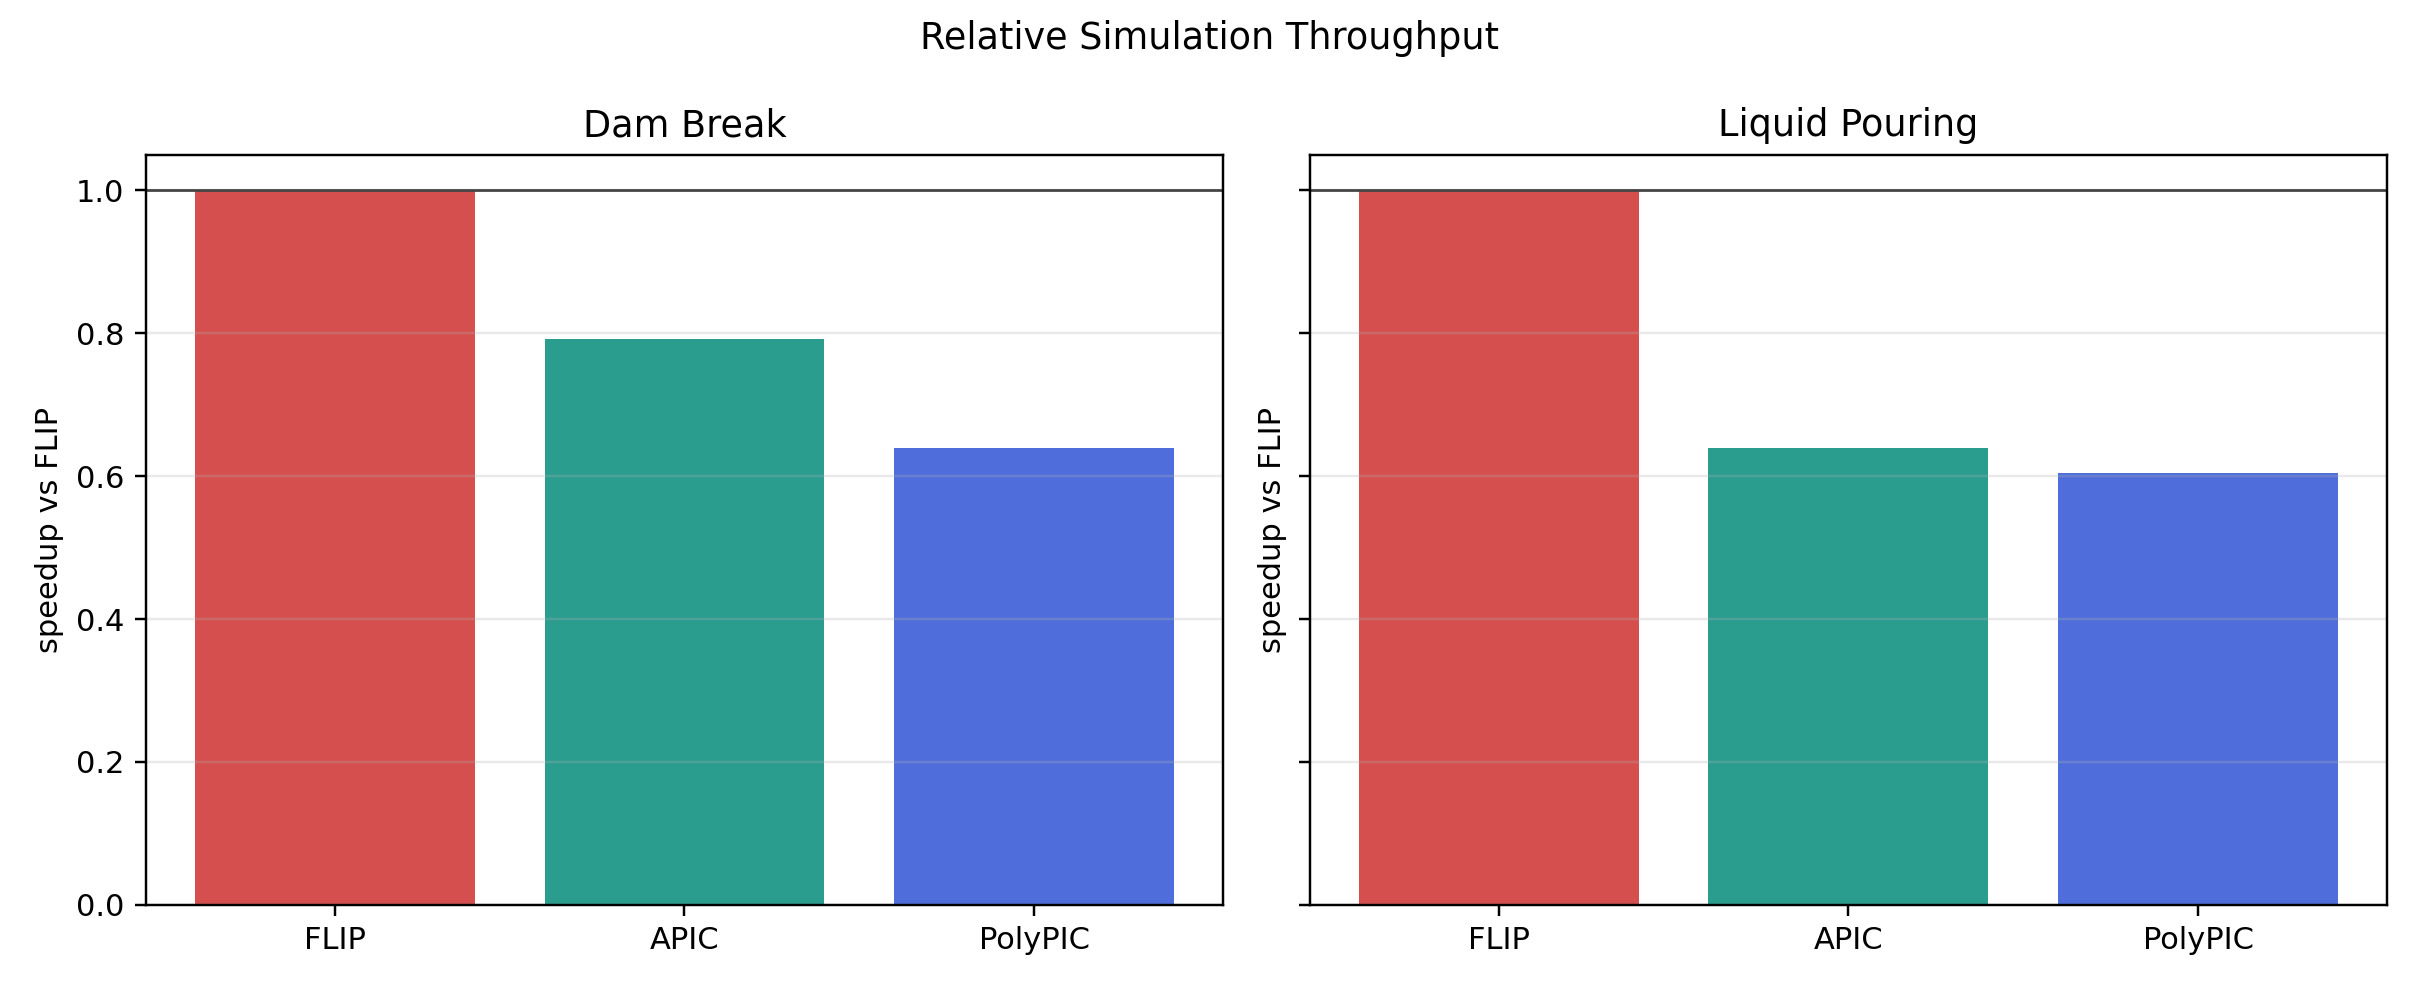
\includegraphics[width=\linewidth]{speedup_vs_flip.png}
  \caption{Relative speedup normalized against FLIP within each scene. Values below $1$ indicate slower runtime than the FLIP baseline.}
  \label{fig:speedup}
\end{figure}

The efficiency benchmark follows the expected method-complexity ordering. FLIP is fastest in both scenes because it transfers only the baseline particle velocity state. APIC is slower because it carries and updates affine velocity information. PolyPIC is slowest because its higher-order local transfer stores and evaluates more particle-side information. Relative to FLIP, APIC reaches $0.79\times$ speed on dam break and $0.64\times$ speed on liquid pouring, while PolyPIC reaches $0.64\times$ and $0.60\times$, respectively.

\FloatBarrier

\section{Discussion}

The experiments support four observations. First, a shared framework is essential: small changes in resolution, particle count, or boundary treatment can dominate the numerical differences between transfer schemes. Second, kinetic energy is informative but not sufficient on its own. Higher energy can indicate useful reduced dissipation, but it can also expose transfer noise or excessive momentum retention. Third, APIC and PolyPIC require more implementation care than baseline FLIP; APIC in particular needed affine-matrix limiting to avoid NaN growth in full runs. Fourth, richer transfer state has measurable runtime cost, as shown by the controlled benchmark.

For dam break, PolyPIC gives the clearest advantage in integrated kinetic energy. For liquid pouring, APIC and PolyPIC are smoother and more restrained than FLIP, with PolyPIC retaining slightly more energy than APIC while remaining stable. These observations are consistent with the motivation behind affine and polynomial transfers: additional local velocity information can improve transfer quality, but a compact implementation must still manage stability and throughput.

\section{Limitations}

This is a small-scale validation rather than a production simulator benchmark. The renderer is particle-based and does not include a high-quality surface reconstruction stage. The runtime benchmark is simulation-only; rendering and video export are excluded, and the first five frames are discarded. This makes the timing comparison more controlled than the original rendered frame times, but it still measures this implementation, these scenes, and this hardware configuration rather than a hardware-independent property of the algorithms.

The experiment set is also intentionally narrow: it contains two scenes, one grid resolution, one particle-generation policy, and one FLIP/PIC blend ratio. The APIC implementation includes damping and finite-value guards for robustness, so its measured energy behavior is not an idealized APIC-only result. A larger study could sweep resolution, source strength, CFL settings, and transfer parameters.

\section*{Tool Use Statement}

Large language models assisted with implementation debugging, batch-command preparation, plotting code, and language editing. All numerical values in the tables and figures are computed from the committed simulation outputs.

\begin{thebibliography}{00}

\bibitem{brackbill1986flip}
J.~U. Brackbill and H.~M. Ruppel, ``FLIP: A method for adaptively zoned, particle-in-cell calculations of fluid flows in two dimensions,'' \emph{Journal of Computational Physics}, vol.~65, no.~2, pp. 314--343, 1986, doi:10.1016/0021-9991(86)90211-1.

\bibitem{foster2001liquids}
N.~Foster and R.~Fedkiw, ``Practical animation of liquids,'' in \emph{Proceedings of SIGGRAPH 2001}, pp. 23--30, 2001, doi:10.1145/383259.383261.

\bibitem{zhu2005sand}
Y.~Zhu and R.~Bridson, ``Animating sand as a fluid,'' \emph{ACM Transactions on Graphics}, vol.~24, no.~3, pp. 965--972, 2005, doi:10.1145/1073204.1073298.

\bibitem{jiang2015apic}
C.~Jiang, C.~Schroeder, A.~Selle, J.~Teran, and A.~Stomakhin, ``The affine particle-in-cell method,'' \emph{ACM Transactions on Graphics}, vol.~34, no.~4, Article 51, 2015, doi:10.1145/2766996.

\bibitem{fu2017polypic}
C.~Fu, Q.~Guo, T.~Gast, C.~Jiang, and J.~Teran, ``A polynomial particle-in-cell method,'' \emph{ACM Transactions on Graphics}, vol.~36, no.~6, Article 222, 2017, doi:10.1145/3130800.3130878.

\bibitem{hu2019taichi}
Y.~Hu, T.-M. Li, L.~Anderson, J.~Ragan-Kelley, and F.~Durand, ``Taichi: A language for high-performance computation on spatially sparse data structures,'' \emph{ACM Transactions on Graphics}, vol.~38, no.~6, Article 201, 2019, doi:10.1145/3355089.3356506.

\bibitem{bridson}
R.~Bridson, \emph{Fluid Simulation for Computer Graphics}, 2nd ed. CRC Press, 2015.

\end{thebibliography}

\end{document}
